\chapter{Calibrations}\label{chap:calibration}

\acl{BBCEAS} has a simpler setup and lower cost in comparison to \ac{CRDS}, but
\ac{BBCEAS} does require a few calibration procedures in order to acquire
accurate absorption spectra. The basic calibrations that should be done with a
\ac{BBCEAS} instrument are: a measurement of the absorption limits where the
signal is linear, an analysis of the error of the detected intensity signal,
and the reflectivity of the mirrors used for the optical cavity.

To find the absorption coefficient values under which an \ac{BBCEAS} experiment
results in a linear correlation with concentration, it is common to test the
instrument using a strong absorber. One such absorber is rhodamine 6G, a dye
that can be used to create a laser \cite{Pappalardo:1970hi} or as a fluorescent
marker \cite{Gear:1974tf}.

The error in the detection of the intensity comes down to two important
sources: the error in the \ac{CCD} and the intensity fluctuation over time of
the light source. The intensity fluctuations are especially important, as it is
possible -- and in some cases, extremely likely -- for the intensity of the
light entering the cavity to change between the measurement of the blank and
the measurement of the sample. This fluctuation at best provides a false
understanding of the detection limit of the setup and, in the case of high
variability in the input source, silently modulates the absorption peaks in
acquired spectra.

Finally, the mirror reflectivity is required for any of the equations of the
absorption coefficient or its standard deviation. Giving a guess on the mirror
reflectivity at a particular wavelength based on the average mirror
reflectivity can lead to inaccurate absorption coefficient calculations and
alter the shape of the calculated spectrum \cite{Berden:2009wk}. This case is
more common than one may expect, as the multiple layers of thin films deposited
on the mirror's surface introduces characteristic ripples in the mirror
reflectivity as a function of wavelength \cite{Islam:2007ea}.

This chapter will discuss these calibrations for the stated problems to
characterise the \ac{BBCEAS} instrument used in this report.



\section{Limits of linearity using Rhodamine 6G}\label{sec:rhodamine}

There are two important considerations for regions where the concentration of
rhodamine correlates linearly with the concentration of an absorber. One
consideration is the calculation of absorption using $A = \alpha  l$, where $l$
is the path length when considering multiple passes through the cavity.  It is
possible to measure an $\alpha$ value that leads to an absorption of greater
than one, which has no physical meaning.

\begin{figure}
\begin{center}
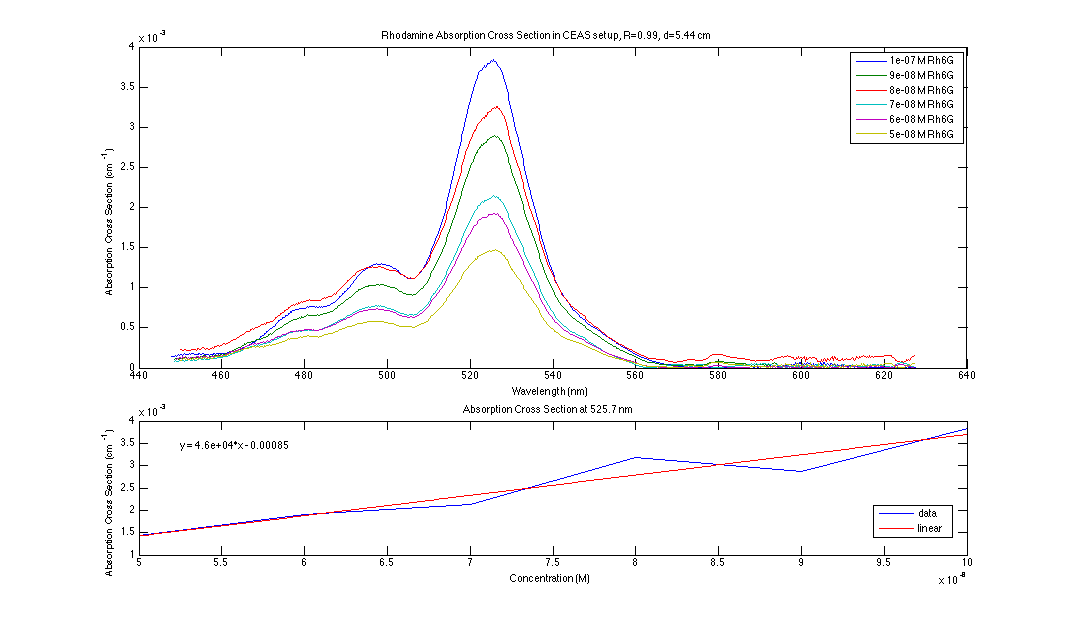
\includegraphics[width=\textwidth]{figures/Rh6G_absorption_cross_section_and_linearity}
\end{center}
\caption{Rhodamine 6G Spectrum from \ac{BBCEAS} measurement}
\label{fig:rh6g}
\end{figure}


While the upper bound to the linearity of the \ac{BBCEAS} equation is useful
for determining when experimental results may be strange, a tighter bounding
set is useful to determine what sorts of concentrations would be best measured
by the \ac{BBCEAS} technique. Unfortunately, the only way to measure where
absorption coefficients correlate linearly with concentration is to acquire
spectra from many different concentrations and plot the absorption at the peak
wavelength as a function of concentration.\marginpar{Get linearity figure}
This is shown in Figure~\ref{fig:rh6g_lin}.

\begin{figure}
\begin{center}
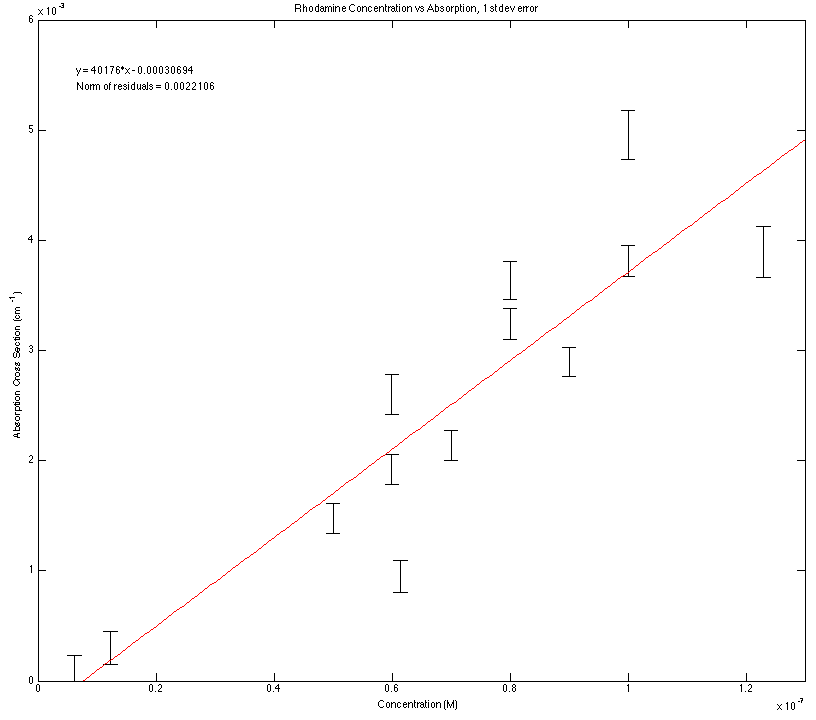
\includegraphics[width=\textwidth]{figures/rhodamine_concentration_vs_conc_linear.png}
\end{center}
\caption{Linearity in Rh6G \ac{BBCEAS} measurement. After this region, the collected data took on a cubic trend.}
\label{fig:rh6g_lin}
\end{figure}

\begin{figure}
\begin{center}
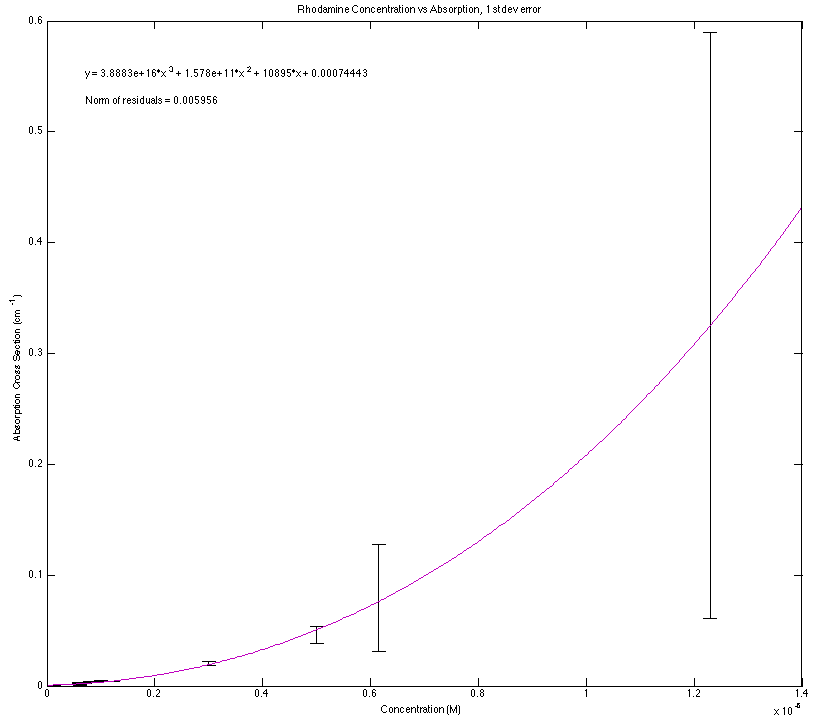
\includegraphics[width=\textwidth]{figures/rhodamine_concentration_vs_conc_non_linear.png}
\end{center}
\caption{Non linearity in Rh6G \ac{BBCEAS} measurement. The fitted line is a cubic trend.}
\label{fig:rh6g_nonlin}
\end{figure}

As can be seen in figure~\ref{fig:rh6g_nonlin}, the lower the concentration, the
better we can fit a linear regression to the data acquired. As such, a lower
bound is better defined as the limit of detection, instead of attempting to
extrapolate a linear function to below the noise levels of the instrument.

One problem with absorption spectroscopy techniques is that the dynamic range
is mainly dependent on the absorber. Strong absorbers will have smaller
concentrations where the calculated absorption coefficient is linear. Weak
absorbers have an advantage is greater detection ranges under this regime, but
suffer from a lower sensitivity to the concentration as small changes in
intensity correlate to larger changes in concentration, in comparison to strong
absorbers.

As a guide to the detectable concentration ranges, it is possible to calculate
the molar emissivity $\epsilon$ range of a \ac{BBCEAS} setup by dividing the
absorption coefficient value by the concentration it represents. Then, if one
knows the molar emissivity of an absorber it is possible to determine a rough
upper bound of the concentration limit of detection. Unfortunately many
substances of interest have unknown or poorly characterised absorption spectra
in terms of molar emissivity in the liquid phase, and there is no convenient
methods of determining valid concentration ranges.

\section{Intensity Fluctuations in BBCEAS measurements}\label{sec:light_fluc}

%% TODO Add section intro here.

\subsection{Intensity fluctuations due to light source stability}\label{subsec:laser_fluc}

\begin{figure}[h!]
\begin{center}
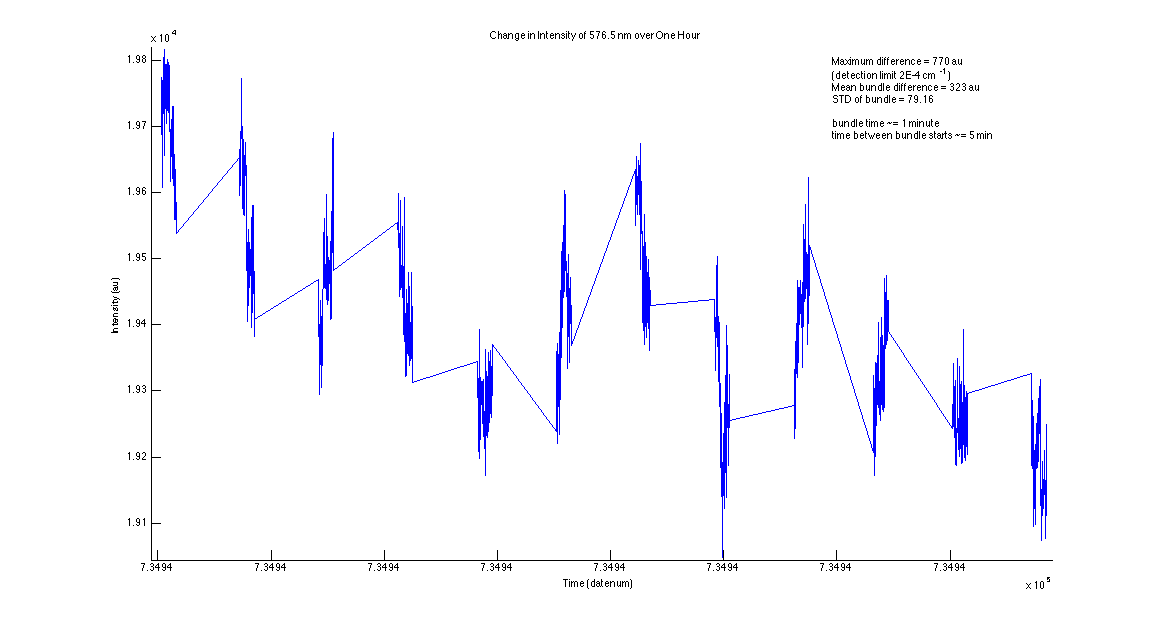
\includegraphics[width=\textwidth]{figures/change_in_intensity_of_576_5nm_over_one_hour.png}
\end{center}
\caption{Laser Fluctuation over time}
\label{fig:laser_fluc}
\end{figure}

\ac{BBCEAS} measurements, while based on \ac{CRDS}, do not share the benefit of
being immune to intensity fluctuations in the source \cite{Berden:2009wk}. This
is because \ac{CRDS} takes the measurement of the intensity of an individual
pulse of light, whereas \ac{BBCEAS} measures the average steady state ring down
intensity, which represents an average of the light intensity ring down times
across multiple pulses (for pulsed wave sources) or effectively infinite pulses
(for continuous wave sources).

Figure~\ref{fig:laser_fluc} illustrates the problem of light source
fluctuation. In this figure, each ``bundle'' represents approximately the
noise from the \ac{CCD}. If one considers this to bundle to represent the
width of the noise distribution due to the \ac{CCD}, then two different
phenomena can be seen from this figure.

The most obvious is that over time, the intensity error fluctuates in both a
high frequency range (mostly the \ac{CCD} noise) and a lower frequency. This
lower frequency is a result of the drift in the intensity of the output of the
supercontinuum laser. As such, it is simple to see that even a measurement
within five minutes of the blank sample is prone to intensity fluctuation
error.

The second problem with the laser fluctuation is that while most of the high
frequency noise is due to the \ac{CCD}, the stretching of the bundles suggests
that there is a high frequency noise component of the supercontinuum source as
well. This means that the fluctuation of the light source skews the
distribution due to the \ac{CCD} noise, sometimes broadening the width (such as
in the second, third and eighth bundles) and sometimes compressing the noise
distribution (as seen in the second to last bundle).

Combined, these two effects of the intensity fluctuation of the laser lead to
errors in calculating $\alpha$ due to drift between measurements and
$\sigma_{\alpha}$ due to fluctuations in $\sigma_{I}$ and $\sigma_{I_0}$. An
additional frustration arises when one considers that these fluctuations in
intensity are often wavelength dependent, so it is not simple to extrapolate
the error calculations in intensity from one wavelength to another.

If the blank and sample spectra are taken within a few minutes of each other,
these error effects are minimised, but still lead to unaccountable error in the
final absorption spectrum. Given that the calculation of the standard
deviations will take part of the high frequency noise into account, and the
fast acquisition will minimise the low frequency source of noise, for most
measurements one can scrape by with these sources of error. However, for a
better sensitivity, information about the light source fluctuation over time is
required to remove the laser noise. Without this information, it is impossible
to give a true estimate of the sensitivity of a \ac{BBCEAS} instrument.

\subsection{Intensity fluctuations as a result of turbulence}

\begin{figure}
\begin{center}
\includegraphics[width=\textwidth]{figures/water_relax.pdf}
\end{center}
\caption{Relaxation time inside the cuvette}
\label{fig:relax}
\end{figure}

An additional source of error that causes intensity fluctuations is, perhaps
surprisingly, the turbulence of the solution. This can be clearly seen in
Figure~\ref{fig:relax}, where the intensity detected fluctuates wildly during
the injection of liquid into the cuvette (for this figure, water was injected
into a cavity containing water). One will notice that right after the injection
phase, the intensity value reaches a maximum, falls and then slowly builds back
up to the beginning level.

The fluctuation and slow build up is due to the alignment of the light within
the cavity. Any optical cavity is very sensitive to deflections of any sort.
The turbulence in the cuvette seems to deflect the path of the light slightly.
This disrupts the measured intensity by changing the total build up intensity
of light within the cavity and by changing the coupling efficiency of the
resulting light with the fibre based grating spectrometer.

Luckily, once the injection of liquid has ceased, the resulting intensity build
up is modelled extremely well by an exponential rise back to the default
value. Using this type of model, it is simple to calculate that for the
\ac{BBCEAS} design used in this report, the time required to wait after an
injection is approximately one minute.
Knowing this time constant, and the slow fluctuation of the light source over
time, we can predict an approximate window in which the highest quality,
lowest noise spectra are likely to be taken.

\section{Mirror Reflectivity}\label{sec:mirror_considerations}

\begin{figure}
\begin{center}
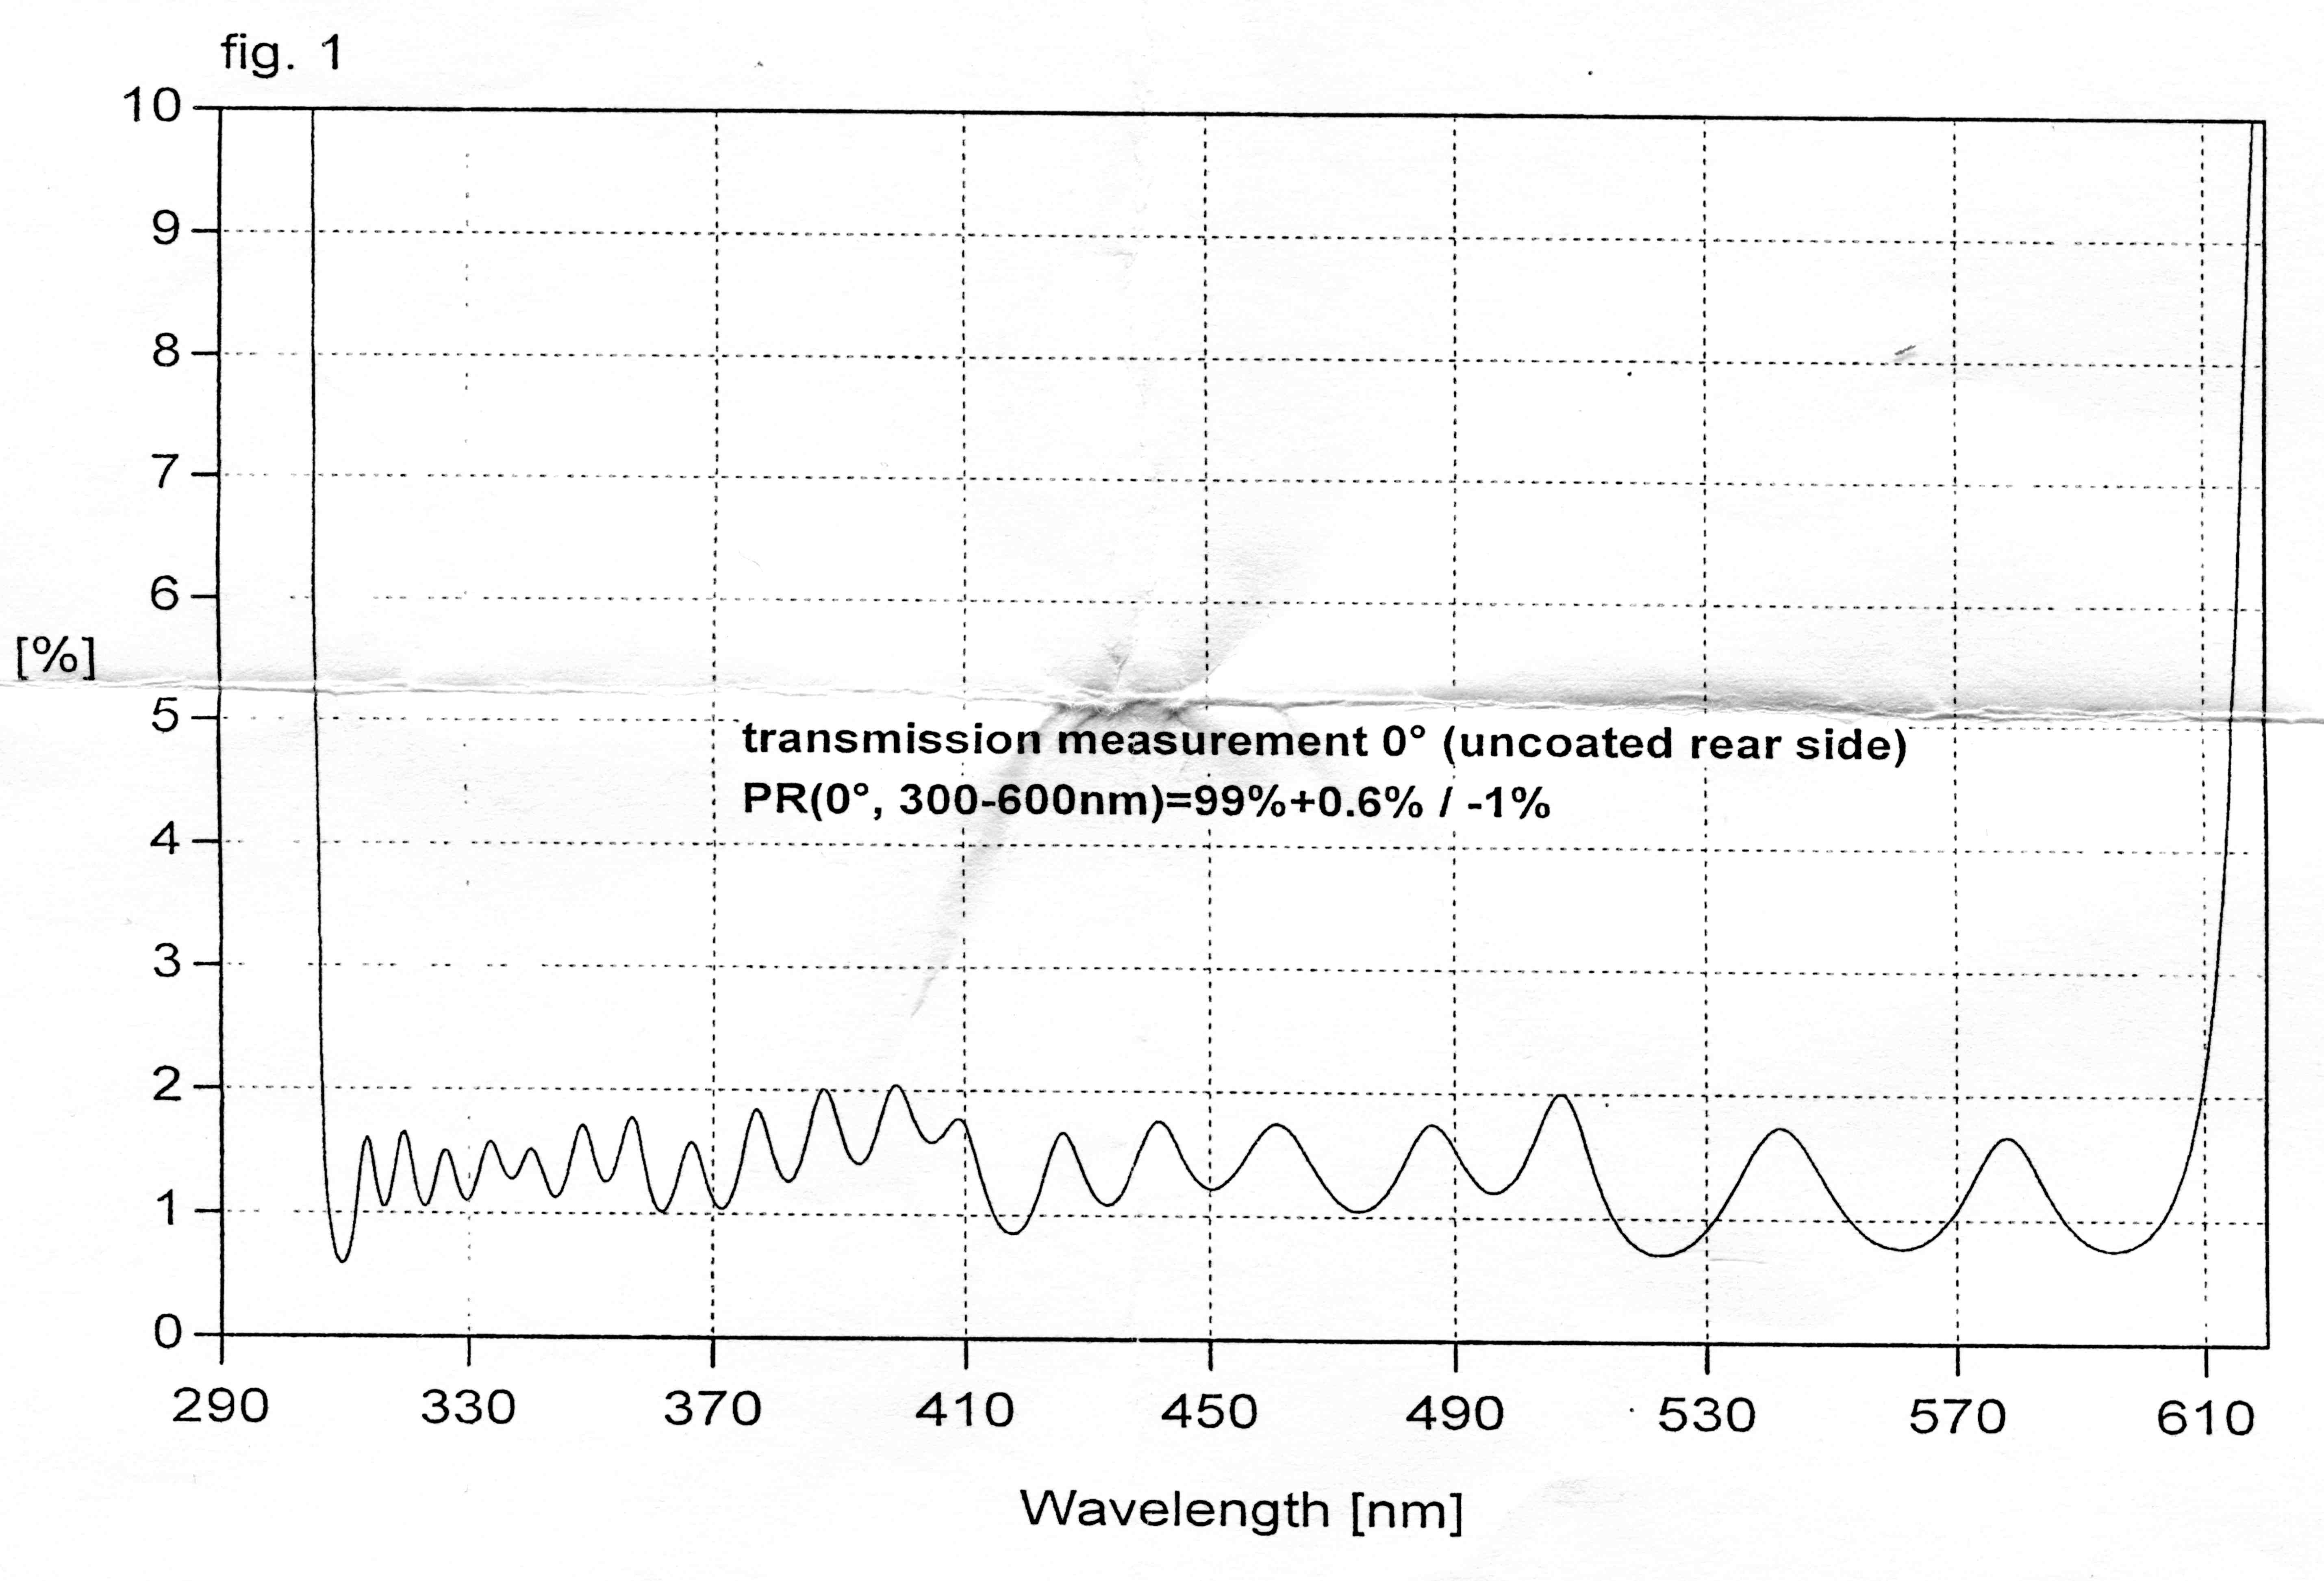
\includegraphics[width=\textwidth]{figures/mirrors.jpg}
\end{center}
\caption{The mirror reflectivity provided by the manufacturer.}
\label{fig:mirror}
\end{figure}

No matter what \ac{BBCEAS} equation an experimenter decides to use to calculate
the absorption spectrum of a sample, the mirror reflectivity must be explicitly
known, as it appears in the form of $\tfrac{1-R}{d}$ \eqref{eq:ceas_std} or in
multiple places for other equations \eqref{eq:ceas_geo_mod}. The inclusion of
$R$ in these equations represents a correction to the path length to account
for the number of passes that light undergoes once it is inside the cavity.

If one neglects to determine the mirror reflectivity of the cavity, as a
function of wavelength, then two anomalous actions occur. The simplest to
understand is that the calculated values of absorption can have an extra error
that can easily exceed error due to other sources. While a calibration against
a known concentration allows one to neglect this source of error when
attempting to determine the unknown concentration of an absorber, the values
calculated provide an inaccurate understanding of the actual absorption of a
particular electronic transition.

The second, more peculiar result of neglecting the mirror reflectivity curve is
that the calculated absorption spectrum changes in \emph{shape}, which  can
lead to both artifacts in the spectrum as well as an alteration of the shape of
a transition. Attempting to fit an accurate profile to a transition in a
spectrum would be an exercise in frustration at best.

There are two ways to determine the mirror reflectivity curves. The first is
to simply have the manufacturer provide the information, or to digitalise a
graph provided through an \ac{FTS} type measurement, although this is known to
not work very well in practice as the mirror reflectivity is a function of the
alignment of the cavity \cite{Berden:2009wk}. The second common method is to
use the \ac{BBCEAS} setup in a \ac{CRDS} experiment, which, due to the self
calibrating nature of \ac{CRDS}, allows one to extract the mirror reflectivity
curves.



\section*{Chapter Review}

While \ac{BBCEAS} does require a few calibration steps to acquire a full
understanding of the spectra it produces, these procedures are not unlike what
an experimenter would go through for a normal absorption, single pass
measurement. In addition, these considerations increase the information of
absorption spectra by characterising the noise inherent in the instrument at
each wavelength the instrument measures at, correcting for the nonlinear
effects that can occur during a measurement.
